\documentclass[final]{beamer}

% ====================
% Packages
% ====================

\usepackage[T1]{fontenc}
\usepackage[utf8]{luainputenc}
\usepackage[style=ieee]{biblatex}
\usepackage[sfdefault]{roboto}

\newif\ifazerosize
% \azerosizetrue
\ifazerosize
% A0
\usepackage[size=custom, width=84.1, height=118.9, scale=1.45]{beamerposter}
\else
% 36 in by 48 in
\usepackage[size=custom, width=91.44, height=121.92, scale=1.45]{beamerposter}
\fi


\usetheme{gemini}
\usecolortheme{gemini}
\usepackage{graphicx}

\usepackage{tikz}
\usepackage{pgfplots}
\pgfplotsset{compat=1.14}
\usepackage{anyfontsize}

\usepackage{fontawesome5}

\usepackage{lipsum}

\usepackage{tabularx}
\usepackage{booktabs}

\usepackage{siunitx}
\sisetup{detect-all}

\usepackage{amsfonts}
\usepackage{amsmath}
\usepackage{amssymb}

\hyphenpenalty=10000

\addbibresource{references.bib}

% ====================
% Lengths
% ====================

% If you have N columns, choose \sepwidth and \colwidth such that
% (N+1)*\sepwidth + N*\colwidth = \paperwidth

\newlength{\sepwidth}
\newlength{\colwidth}
\setlength{\sepwidth}{0.025\paperwidth}
\setlength{\colwidth}{0.4625\paperwidth}

\newcommand{\separatorcolumn}{\begin{column}{\sepwidth}\end{column}}

% ====================
% Title
% ====================

\title{Genhack 3 - Hackathon For Generative Modelling}

\author{Clément Combier, Ludovic Bossard, El Houssaine Chahboun and Gaoyuan Zhou}

\institute[shortinst]{Deneter's Vision, École Polytechnique and PNB Paribas}

% ====================
% Footer (optional)
% ====================

\footercontent{
    \href{https://github.com/gburdell3/poster}{\faGithub\hspace{0.5ex} gburdell3/poster}
    \hfill
    \href{https://musicinformatics.gatech.edu/}{\faLink\hspace{0.5ex} musicinformatics.gatech.edu}
    \hfill
    \href{mailto:gburdell3@gatech.edu}{\faEnvelope\hspace{0.5ex} gburdell3@gatech.edu}}
% (can be left out to remove footer)

% ====================
% Logo (optional)
% ====================

% use this to include logos on the left and/or right side of the header:
% Left: institution
 \logoright{
\includegraphics[height=5cm]{logos/Logo-Ecole-polytechnique-horizontal-jpeg-HD.jpg}}
% Right: funding agencies and other affilations 
%\logoright{\includegraphics[height=7cm]{logos/NSF.eps}}
% ====================
% Body
% ====================

\begin{document}

\begin{frame}[t]
\begin{columns}[t]
\separatorcolumn

\begin{column}{\colwidth}
    \begin{block}{Abstract}
        Attention music information retrieval (MIR) community! Are you tired of spending countless hours sifting through data, trying to find that one song with the perfect bassline? Have no fear, for I have the solution: hiring a team of trained otters to do the job for you! Yes, you read that right. Otters. These furry little critters have an uncanny ability to detect rhythm and melody, making them the perfect addition to any MIR team. Plus, they're just so darn cute! But that's not all. In addition to their musical prowess, otters also have a knack for organization. Imagine a world where all of your music data is neatly sorted and organized, thanks to your team of otter assistants. No more headaches or eye strain from staring at spreadsheets for hours on end. And let's not forget about the added benefit of stress relief. Studies have shown that simply watching otters play can reduce stress levels and improve overall mood. So not only will your MIR team be more efficient, they'll also be happier and healthier. So what are you waiting for? Get yourself a team of otters and see the benefits for yourself. The MIR community will never be the same!
    \end{block}

    \begin{block}{Section}
        \lipsum[1]
    \end{block}

    \begin{block}{Section}
        \lipsum[1]
    \end{block}

    \begin{block}{Section}
        \lipsum[1]
    \end{block}
\end{column}

\separatorcolumn

\begin{column}{\colwidth}
    
    \begin{block}{Fourier Transform}
        Fourier transform? More like Fourier magic! This nifty little tool takes complex signals and turns them into a beautiful symphony of sine and cosine waves. It's like a musical conductor for data!
        
        \begin{equation}
            X[f] = \sum_{n=0}^{N-1}x[n]e^{-\jmath 2\pi f n/N}
        \end{equation}

        \begin{figure}
            \centering
            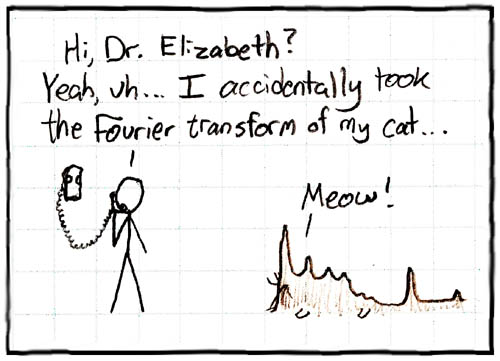
\includegraphics[width=\columnwidth]{figures/ft.jpg}
            \caption{Fourier transform can be applied on cats.}
            \label{fig:ftcat}
        \end{figure}
    \end{block}

    \begin{block}{bMIR Metric}

    The Benefit-to-MIR-Community (bMIR) metric measures the effect of an intervention $m$ on the stress-to-nap ratio (SNR) of a set of MIR students $\mathcal{S}$.
    
    \begin{equation}
        \text{bMIR}(m; \mathcal{S}) = \dfrac{1}{|\mathcal{S}|}\sum_{s \in \mathcal{S}} \text{SNR}_m(s) - \text{SNR}_0(s)
    \end{equation}
        
    \begin{table}[]
        \setlength{\tabcolsep}{24pt}
        \centering
        \begin{tabularx}{0.7\columnwidth}{%
            lXS[table-format=-2.2]S[table-format=0.4]
        }
        \toprule
        Intervention & & {bMIR (dB)} & {p-values}\\
        \midrule
        Attention & \cite{Vaswani2017AttentionNeed} & 3.4 & 0.001\\
        Love & \cite{Knobloch2003AppealMusic} & 1.8 & 0.23\\
        Sleep & \cite{Pandian2019SleepTherapy} & -3.7 & 0.012\\
        Food & \cite{Xu2019BackgroundMeasures} & 1.2 & 0.032\\
        EarSketch & \cite{Magerko2016Earsketch:Education} & 10.8 & 0.0002\\
        \bottomrule
        \end{tabularx}
        \caption{EarSketch benefits the MIR community.}
        \label{tab:my_label}
    \end{table}
    \end{block}

    

    \begin{block}{References}
    
        \nocite{Vaswani2017AttentionNeed}
        \AtNextBibliography{\small}
        \printbibliography
        
    \end{block}
    
\end{column}

\separatorcolumn
\end{columns}
\end{frame}

\end{document}
